% !TeX spellcheck = hu_HU
% !TeX encoding = UTF-8
\chapter{Kapcsolódó munkák}\label{sec:kapcsolodo}

\section{Gráf adathalmazok lekérdezése}
\paragraph{Cypher}
A Cypher nyelvhez elérhető a \emph{Cypher for Apache Spark}\footnote{\url{https://github.com/opencypher/cypher-for-apache-spark}} projekt, ami a népszerű Spark keretrendszeren futtatható programokra képez le openCypher lekérdezéseket. A Cypher for Apache Spark projekt megoldása a Spark adatfolyam-orientált (streaming) programozási modellje miatt nem alkalmas módosítás és törlés műveletek kezelésére.

\paragraph{G-CORE}
A G-CORE~\cite{DBLP:conf/sigmod/AnglesABBFGLPPS18} az LDBC Graph Query Language munkacsoportjának és több cég közreműködésével tervezett lekérdezési nyelv a tárolt utakkal rendelkező tulajdonsággráfokhoz (path property graph). Ebben az adatmodellben az éleken túl lehetőség van utak és azok tulajdonságainak tárolására is. A G-CORE lehetőséget nyújt az utak és tulajdonságaik lekérdezésére, módosítására. A G-CORE tervezésére befolyással volt a Cypher nyelv, így a szemantikai hasonlóságok mellett sok konstrukció azonos szintaxissal definiálható.

\paragraph{Datalog}
A Datalog egy deklaratív programozási nyelv, amely szintaktikailag a Prolog nyelv részhalmaza. Datalogban sor- és oszlopkalkulushoz hasonló lekérdezéseket lehet megfogalmazni. Számos kiterjesztése létezik, amelyeket különböző adatbázis-kezelőkben használnak, például LogiQL nevű kiterjesztését a LogicBox adatbázis-kezelőben~\cite{DBLP:conf/sigmod/ArefCGKOPVW15}.

\paragraph{VIATRA Query Language}

A gráfmintaillesztést széles körben használják a modellvezérelt technológiákban, például a \viatra keretrendszerben~\cite{DBLP:journals/sosym/VarroBHHRU16}. A keretrendszer saját lekérdezőnyelve egy Dataloghoz hasonló nyelv, a \vql (VQL), amely támogatja a gráfminták komponálását, a rekurzív minták megfogalmazását és az aggregációt. A \viatra keretrendszer a Rete algoritmust használja a gráfmodellek hatékony ellenőrzésre és transzformációjához. Az \iqd egy elosztott inkrementális gráflekérdező~\cite{DBLP:conf/models/SzarnyasIRHBV14}, amely lekérdezőnyelve a VQL-en alapul és RDF gráfok lekérdezését teszi lehetővé.

A \viatra egy korábbi verziójában készült egy prototípus alkalmazás~\cite{DBLP:conf/gg/BergmannHH12}, ami inkrementális gráftranszformációt végez relációs adatbázisokon. A prototípus  gráfmintákból SQL lekérdezéseket készít a kezdeti illeszkedési halmazok meghatározásához. Egy mintát egy több illesztést tartalmazó, lapos SQL lekérdezéssé képez le. Ezután az illeszkedési halmazokat az adatbázis triggereinek (adott esemény hatására lefutó SQL kifejezések, például sorok beszúrása, törlése vagy módosítása) használatával tartja karban.



\section{Teljesítménymérési keretrendszerek gráflekérdezésekre}

A dolgozat készítése során több teljesítménymérési keretrendszert tanulmányoztam, amelyek lehetővé teszik gráf információs rendszerekben futtatott lekérdezések teljesítményének vizsgálatát. Az általam fontosnak vélt keretrendszerek legmeghatározóbb tulajdonságait mutatom be ebben a fejezetben.

\paragraph{LDBC Semantic Publishing Benchmark}
Az LDBC egy másik teljesítményérési keretrendszere a Semantic Publishing Benchmark~\cite{DBLP:conf/semweb/KotsevMPEFK16} (SPB), amely a British Broadcasting Corporation\footnote{\url{http://www.bbc.com/}} (BBC)  Dynamic Semantic Publishing rendszeréhez hasonló RDF adathalmazt használ. Az adathalmazban különböző kreatív munkák (cikkek, fényképek és videók) érhetőek el különböző szempontok szerint csoportosítva. A teljesítménymérés során párhuzamosan futnak szerkesztői módosítások, beszúrások és a felhasználói lekérdezések az állandó terhelést szimulálva. A mérés során az LDBC SNB-hez hasonlóan az adatbázis-kezelők hatékonyságát leíró jellemzőket rögzít.

Azon túl, hogy csak RDF adathalmaz generálására alkalmas, az LDBC SPB a teljesítménymérés során olyan csak RDF-ben elérhető funkciókat használ, mint a következtetés (\textit{inferencing}), azaz a meglévő kapcsolatok és előre definiált szabályok alapján új kapcsolatok létrehozása. A keretrendszer ezen tulajdonsága miatt nem alkalmas tulajdonsággráf alapú vagy relációs adatbázis-kezelők teljesítménymérésére.

\paragraph{Train Benchmark}
A Train Benchmark~\cite{DBLP:journals/sosym/SzarnyasIRV18} a modellvezérelt technológiák által inspirált teljesítménymérési keretrendszer, amely adatmodellje a vasúthálózat és a hozzá kapcsolódó érzékelő és biztosító berendezések hálózatát tartalmazza. Többféle terhelési profilt definiál, több adatmodellt és lekérdezőnyelvet is támogat, köztük az ebben a dolgozatban használtakat is. Az LDBC SNB keretrendszernél azonban kevesebb nyelvi elemet fed le, például nem teszi lehetővé aggregációk, útvonal-kifejezések vagy éleken definiált tulajdonságok teljesítménymérését.

\section{Illesztések optimalizációja gráfadatbázis-kezelőkben}

A relációs adatbázis kezelők elterjedésének köszönhetően az elmúlt évtizedekben egyre hatékonyabb illesztési algoritmusokat dolgoztak ki. A lekérdezések végrehajtási tervének optimalizálása a végrehajtási terv elemei közötti egymásra épülésének (kb. végrehajtási sorrend, amolyan termelő-fogyasztó viszony) -- a szelekciós tényező becsült értékén alapuló -- ekvivalens átalakításain alapszik. A szelekciós tényező egy illesztés esetén az eredményként előálló reláció sorainak számának aránya az alaprelációk Descartes-szorzatának sorainak számához viszonyítva. Formálisan $ s = \frac{|R_1 \joinop R_2|}{|R_1 \times R_2|} $, ahol $s$ a szelekciós tényező, $R_1$ és $R_2$ pedig az illesztés két alaprelációja. Az illesztési sorrend nagyon fontos a hagyományos relációs lekérdezésekben, így egy jó illesztési sorrenddel sokat lehet nyerni, a hiányában bukni. Annak ellenére, hogy a relációs adatbázis kezelőkben az ezen alapuló algoritmusok és módszerek hatékonynak bizonyultak, a gráfadatbázis kezelők tekintetében sok esetben nem bizonyultak megfelelőnek. A problémát a gráfos lekérdezések tulajdonságai, a tipikusan használt gráfminták okozzák, amelyek általában nincsenek jelen a relációs lekérdezésekben, pl. a körkörös gráfminták, vagy az adatok szokatlan eloszlása. 

\begin{figure}[ht]
	\centering
	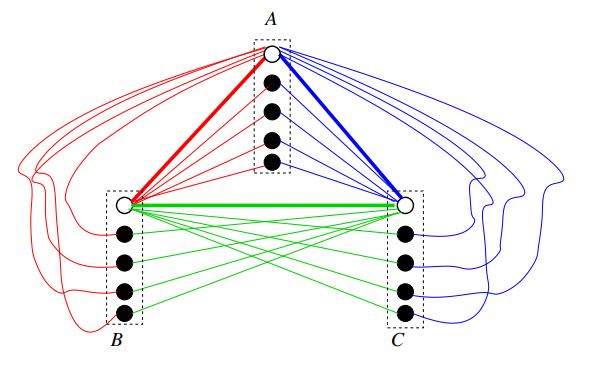
\includegraphics[width=120mm, keepaspectratio]{king}
	\caption{{$\circ$} királyok, {$\bullet$} alattvalók~\cite{DBLP:journals/sigmod/NgoRR13}}
	\label{fig:king}
\end{figure}

\subsection{Körkörös lekérdezés}

A relációs adatbázissal szemben a gráfadatbázisok esetében gyakoriak a köröket tartalmazó lekérdezések. Mivel a relációs adatbázis-kezelőkben a bináris (két alaprelációt tartalmazó) illesztések beváltak, így számos gráfadatbázis is bináris illesztéseket használ az illesztések elvégzésére, köztük a tanszéken fejlesztett ingraph~\cite{DBLP:conf/sdl/MartonSB17} inkrementális gráfadatbázis-kezelő rendszer is. A bináris illesztések rossz teljesítményét \aref{fig:king}.~ábrán látható gráfon mutatom be:
tegyük fel, hogy a három, szaggatott vonallal jelölt királyságban egyik király (üres körök) sem ismeri a saját alattvalóit (teli körök), de minden más királyság összes alattvalóját és a királyukat is ismeri. Ha ebben a gráfban a pontosan 3 darab, páronként különböző színű élt tartalmazó köröket keressük, akkor bináris illesztéseket használva \aref{fig:king_plan}.~ábrán látható végrehajtási tervek egyikét kell végrehajtanunk. Az ábrán \textcolor{red}{\textit{R}}, \textcolor{green}{\textit{S}} és
\textcolor{fullblue}{\textit{T}} az azonos színű élhalmazokat jelentik. Ekkor a második (a végrehajtási terveben legfelső) illesztés alaprelációinak 25 (az első illesztés eredménye) és 9 (a harmadik színű élek) darab sora lesz, az illesztés eredménye pedig 13 darab ($3 \times 4$ darab pontosan kettő királyt tartalmazó kör és 1 darab mindhárom királyt tartalmazó kör) sorból fog állni. Ezek alapján a szelekciós tényező $s = \frac{13}{25 \times 9} \approx 0.058$. Az alacsony szelekciós tényező miatt
ebben az esetben a bináris illesztésnél létezik hatékonyabb módszer is~\cite{DBLP:journals/sigmod/NgoRR13}, a WCOJ (worst-case optimal join) algoritmusok~\cite{DBLP:journals/jacm/NgoPRR18}. Ezek az algoritmusok egyszerre nem kettő, hanem több, akár tetszőleges számú reláció illesztését végzik el egyszerre. Egy ilyen algoritmus a Leapfrog Triejoin~\cite{DBLP:conf/icdt/Veldhuizen14}, ami olyan attribútumok illesztését képes hatékonyan elvégezni, amelyeken értelmezett a rendezés művelet.
A WCOJ algoritmusok kifejezetten az ilyen lekérdezések hatékony végrehajtását segítik. Véleményem szerint \emph{az ingraph teljesítményét jelentősen növelné}, ha a bináris illesztések mellett WCOJ algoritmusokat is megvalósítana.

\begin{figure}[ht]
	\centering
	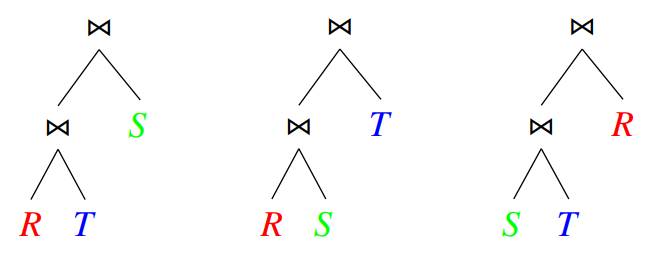
\includegraphics[width=60mm, keepaspectratio]{king_plan}
	\caption{A lehetséges végrehajtási tervek bináris illesztések esetén~\cite{DBLP:journals/sigmod/NgoRR13}}
	\label{fig:king_plan}
\end{figure}

\subsection{Eredmények számosságának becslése}
Mivel az illesztések szelekciós tényezőjének pontos kiszámítása túl költséges művelet, ezért az adatbázis-kezelő rendszerekben gyakran használnak különböző becsléseket (\emph{cardinality estimation}) a szelekciós tényező meghatározására, hogy a lekérdezések végrehajtási tervét ennek figyelembevételével készítsék el.
Az ilyen becslések két nagy csoportba sorolhatóak~\cite{DBLP:journals/vldb/LeisRGMBKN18}:
az \textit{(1)} aggregált adatokon (hisztogramokon) alapuló és
a \textit{(2)} mintavételezésen alapuló becslések.

Az \textit{(1)} esetben az adatbázis-kezelő rendszereknek fel kell építeniük és karban kell tartaniuk az alaprelációkról a szükséges statisztikákat. Ahhoz, hogy az aggregált adatokból megfelelő pontossággal lehessen megbecsülni a szelekciós tényezőt, sok esetben pontosan ismerni kell az adatok struktúráját, esetleg részletesebb statisztikákat kell tárolni és frissíteni. Extrém nagy adathalmazok esetén az is előfordulhat, hogy már a statisztikákat is becslésekkel állítják elő, így növelve a becslés pontatlanságát.

A \textit{(2)} esetben a bemeneti relációk néhány rekordját kiválasztjuk, majd ezek illesztése után az eredeti relációk illesztésének szelekciós tényezőjét becsüljük a kiválasztott elemek szelekciós tényezőjével. A mintavételezésen alapuló eljárások nem követelik meg az adatbázisra vonatkozó statisztikák tárolását és karbantartását, valamint korrelált és nem egységes adatok esetében robusztusak~\cite{DBLP:journals/jcss/HaasNSS96}. Továbbá a mintavétel alapú eljárások lehetővé teszik a becslési hibák értékelését és ellenőrzését. A mintavételezés történhet több lépésben is: minden lépésben kiválasztunk $ n \ge 1$ rekordot mindkét relációból, ezeket illesztjük majd a mintavételezési lépések után azok eredményeit kombináljuk és következtetünk az eredeti illesztés szelekciós tényezőjére. Az egyes lépések után a mintavételezett rekordokat a későbbi lépésekben felhasználhatjuk, vagy akár el is dobhatjuk. A mintavételezési lépések száma lehet egy előre rögzített szám, vagy a mintavételezés folytatódhat addig, amíg egy bizonyos valószínűséget el nem ér a becslés pontossága (azaz amíg nem vagyunk elég biztosak a becslés helyességében).

A gráfadatbázisok egy fontos tulajdonsága, hogy a csúcsok fokszámeloszlása erősen eltolt (skewed).
Míg relációs adathalmazok gyakran normál vagy teljesen véletlenszerű eloszlást követnek,
addig előbbiek általában a hatványtörvény-eloszlást (power law distribution) követik~\cite{Barabasi:2003:ITS}.
A hatványtörvény-eloszlás egy olyan valószínűség-eloszlás, melynek sűrűségfüggvénye
$$ P(X>x)\sim L(x)x^{-(\alpha +1)} $$
alakú, ahol $\alpha > 0$, és $L(x)$ egy lassan változó függvény, amire minden pozitív $r$ esetében igaz, hogy:
$$\lim _{x\rightarrow \infty } \frac{ L(r \cdot x) }{ L(x) } = 1.$$
Egy példa hatványtörvény-eloszlás \aref{fig:powerlaw}.~ábrán\footnote{Forrás: Wikipédia, \url{https://en.wikipedia.org/wiki/Power_law}} látható.
\begin{figure}[ht]
	\centering
	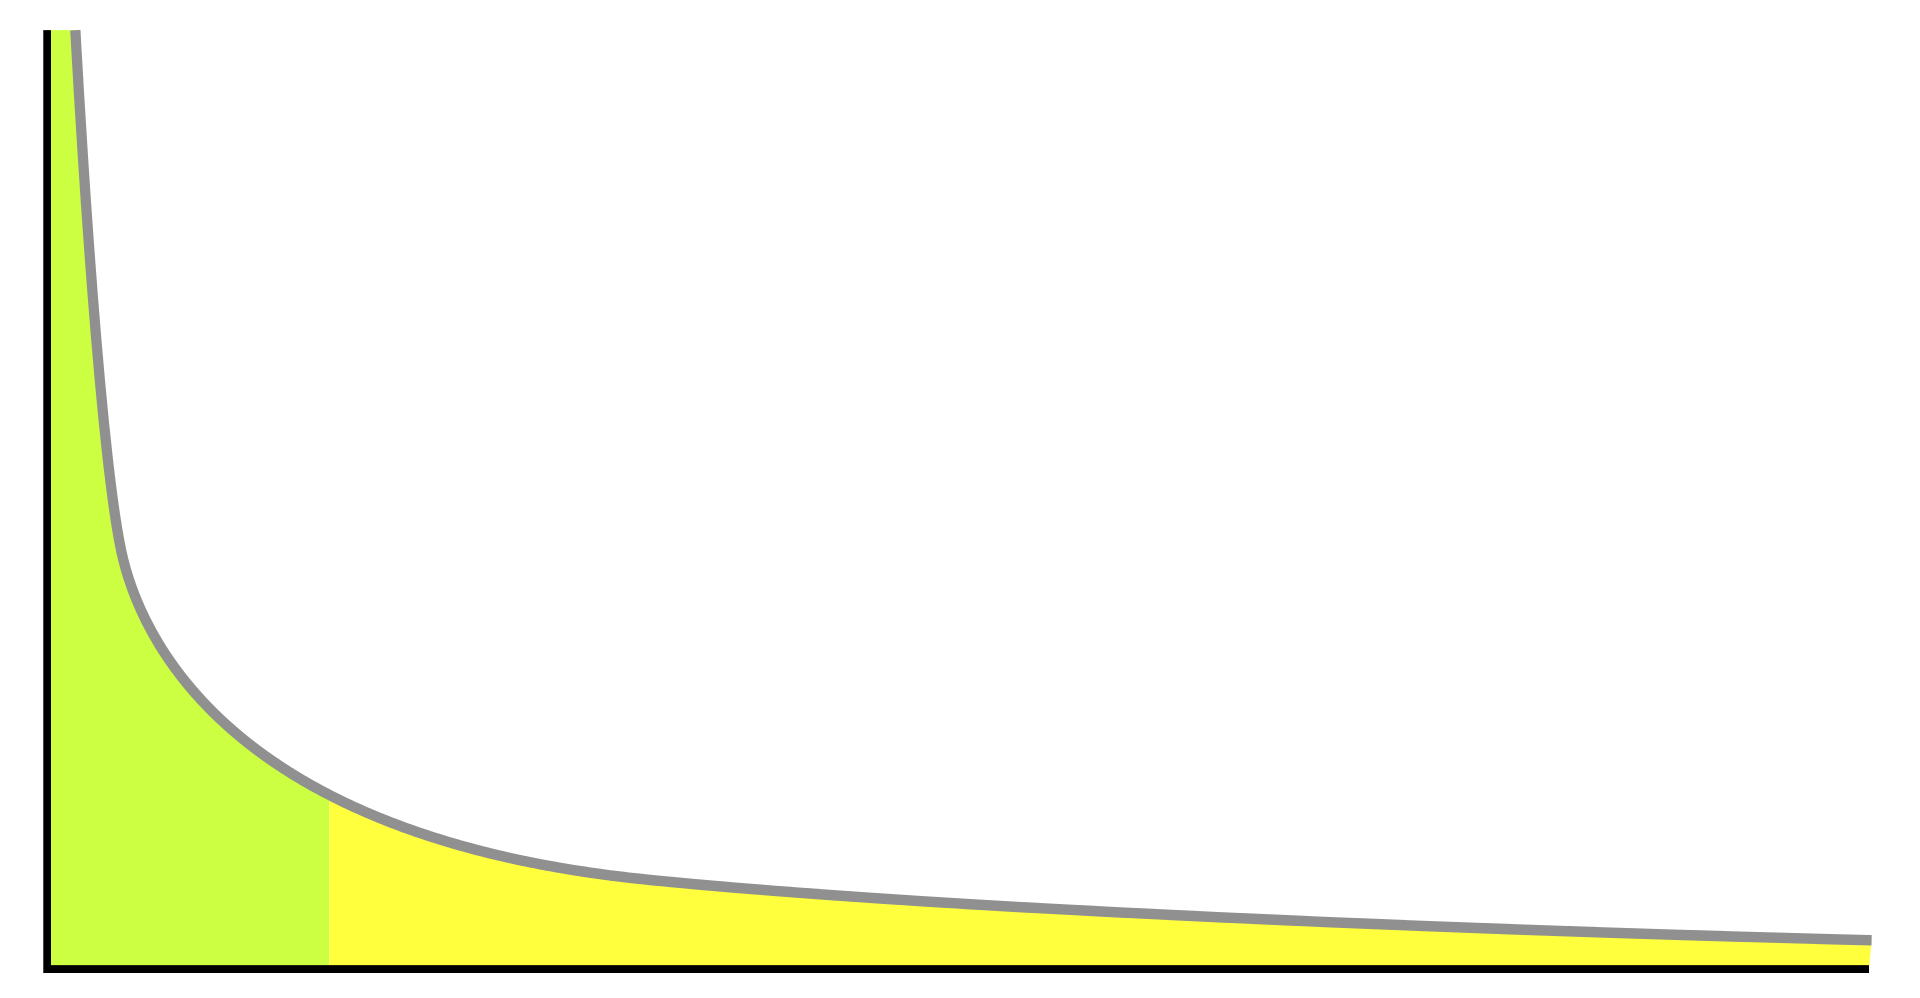
\includegraphics[width=90mm, keepaspectratio]{powerlaw}
	\caption[Egy példa határtörvény-eloszlás]{Egy példa határtörvény-eloszlás, sárgával van jelölve az eloszlás farka (\emph{tail}), zölddel pedig a domináns fej (\emph{head}) rész -- a jól ismert 80-20 szabályhoz hasonlóan.}
	\label{fig:powerlaw}
\end{figure}
\paragraph{Javaslat az ingraph rendszer továbbfejlesztésére}
Ezen ismeretek alapján az ingraph rendszerben szerintem a mintavételezésen alapuló becslési módszert érdemes implementálni, figyelembe véve az \textit{end-biased}~\cite{DBLP:conf/icde/EstanN06} módszert. Ennek a módszernek a lényege, hogy az egyes elemek gyakoriságát nyilvántartja, és az alapján választja ki a mintavételezés során az elemeket. Egy adott $T$ gyakoriság felett minden elemet belevesz a mintába, alatta pedig a gyakoriságával arányos valószínűséggel választja bele a mintába az egyes elemeket. Ez a módszer biztosíthatja, hogy a legmeghatározóbb (leggyakoribb) elemek kiválasztásra kerüljenek, azonban a kevésbé gyakori, azonban összességében az adathalmaz jelentős részét alkotó -- \aref{fig:powerlaw}.~ábrán sárgával jelölt -- elemek közül is megfelelő mennyiségű a mintába kerüljön, így növelve a becslés pontosságát. A módszer lehetőséget biztosít arra, hogy megfelelő hash függvények választásával növeljük annak a valószínűségét, hogy egy adott kulcshoz tartozó elem vagy minden alaprelációban kiválasztásra kerüljön, vagy egyikben sem.

